\chapter[GNSS Overwiev]{\centering \begin{normalsize} \begin{Huge}
			GNSS Overwiev
		\end{Huge} \end{normalsize}}
\label{ch:gnss}

The acronym GNSS\footnote{Global Navigation Satellite Systems} refers to all the satellite systems which allow to define the position of a terrestrial point through the emission of radio signals. The most famous GNSS is NAVSTAR GPS\footnote{NAVigation Satellite Timing And Ranging Global Positioning System}; it was the first installed by USA Department of Defense in 1970s and it is the most widespread. Afterwards, the Russian Federal Government decided to invest in satellite positioning by developing the GLONASS\footnote{GLObal'naja Navigacionnaja Sputnikovaja Sistema} system. In the last years, other countries started to develop their own systems: the European Union presented Galileo and EGNOS\footnote{European Geostationary Navigation Overlay System}, Japan is developing QZSS\footnote{Quasi-Zenith Satellite System}, China is working on BeiDou and India on IRNSS\footnote{Indian Regional Navigational Satellite System}.

Many textbooks present the theory of the GNSS (e.g. \cite{hoffmann2008, Teunissen, Seeber:2003}), and it is not the main purpose of this dissertation to provide a fully detailed description of all these aspects. Nevertheless, this chapter resumes in a non exhaustive way the main concepts on the GNSS positioning with the aim of giving the reader the basic elements to understand the rest of the thesis work.
%Satellite technology is currently named GNSS, referring to the satellites' multi-constellations system
%providing global coverage.


\section{GNSS principles}

GNSS is used to determine the position of a receiver by means of constellations of multiple artificial satellites, knowing the positions of the satellites, namely the ephemerides. The determination of the receiver position, i.e. latitude, longitude and height, relies on the calculated distance from several satellites. Theoretically, from a purely geometrical point of view, the minimum needed number of satellites is three, to solve the three unknowns system. The signals of each satellite allow the user to measure the distance between the receiver and the satellite. This operation is based on two clocks, one on the satellite and one on the receiver, which have totally different time scales: in fact, the receiver's clock starts when the receiver is switched on. This effect is called \textit{synchronisation offset} $\delta t$ and it has to be estimated. Moreover, as widely known, the satellites are equipped with atomic clocks which can be synchronized to the level of nanosecond, but GNSS receivers are typically equipped with less expensive crystal clocks. The synchronisation between the clocks has to be estimated with high precision: a synchronization error of 1 $\mu s$ could lead to a position error in the order of 300 meters. The satellite-receiver distance is calculated on the basis of the signals time of travel $ \tau_{sat,rec}$, using the speed of light $c$:

\begin{equation}
	\rho = c \cdot \tau_{sat,rec}
	\label{eq:pseudorange}
\end{equation}

where $\rho$ is called \textit{pseudorange} because it is affected by synchronisation offset. The introduction of $\delta t$ leads to a system of four unknowns, which must be solved by means of four equations. Thus, to overcome the synchronization problem, a fourth satellite is needed. As a matter of facts, having more than four satellites will not result in a more precise solution, but will just increase the control on the observations, thanks to redundancy.

\section{GNSS segments}

A GNSS is composed by three segments:
\begin{itemize}
	{\item[-] space segment},
	{\item[-] control segment},
	{\item[-] user segment}.
\end{itemize}

\textit{The space segment} consists of many constellations of satellites that are placed above the Earth in nearly circular orbital planes. There are three different orbit altitudes: low Earth orbit (LEO), medium Earth orbit (MEO), and geostationary Earth orbit (GEO) satellites.
The relation between orbit altitude and Earth circulation period is fixed. LEO satellite are located at an altitude of under 2000 km and circulate the Earth in the range of 95 to 120 min. MEO satellites are located at an altitude of 5000 to 20000 km and take about 6 h to circulate the Earth. The altitude of GEO satellites is fixed at 35786 km, in which they exactly match the Earth rotation speed (i.e. circulate the Earth once in 24 hours) and remain exactly at the same point from the Earth view. Each satellite is equipped with devices that are used for navigation or other special tasks. The satellite receives, stores, and processes transmitted information from a ground control center. In order to be recognised, satellites have various identification systems, such as the launched sequence number, the orbital position number, and the system specific name.

\textit{The control segment} is responsible of controlling the whole
system including its deployment and maintenance, tracking of the satellites in their orbits and the clock parameters, monitoring of auxiliary data, and upload of the data message to the satellites. The control segment is also responsible for data encryption and service protection against unauthorized users. Moreover, tracking stations located around the world coordinate the activities for controlling and monitoring the system using bidirectional communication between GNSS satellites.

Finally, the \textit{user segment} consists of all the users equipped with passive receivers, i.e. GNSS receivers and antenna, able to acquire, decode and record the signals coming from satellites.

Figure (\ref{FIG:GNSSsegments}) shows a scheme of GNSS segments.

\begin{figure}[ht] 
	\centering
	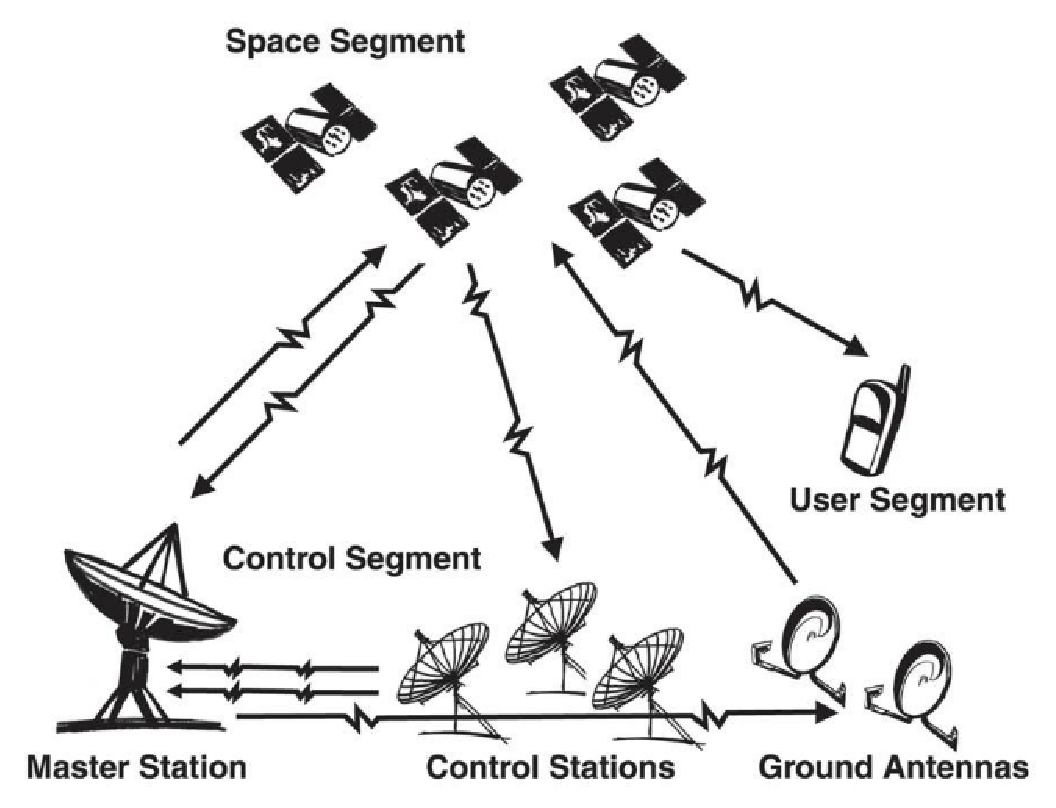
\includegraphics[scale=0.5]{fig/GNSSsegments.eps} 
	\caption{GNSS segments}
	\label{FIG:GNSSsegments} 
\end{figure}

\subsection{GPS}

The NAVSTAR Global Positioning System has been developed by the U.S. Department of Defense for military purpose; the first satellite was launched in 1977 and the system reached its full operational capacity in 1995. Then, in 2000, the U.S. Congress made the GPS available for civilians too, thus, since that time, civilians can access GPS service worldwide free of charge.
The space segment of GPS consists of 24 active MEO satellites, at an altitude of 20200 km, distributed in six equally spaced orbit planes with inclination of $\ang{55}$ on to the Equator. Each satellite circulates the Earth in a period of 12 sidereal hours. The constellation allows the visibility of at least four satellites everywhere and in every time with an elevation of more than $\ang{15}$ on the horizon; this is the minimum requirement for retrieving of the position, but often a higher number of satellites (7 or 8) can be seen. 


%\textcolor{blue}{It is important to underline that the geometrical collocation of the satellites strongly influences the positioning accuracy. The effect of satellites geometry is usually expressed by the DOP\footnote{Dilution Of Precision} index. The different parameters to quantify the goodness of the geometrical configurations are called PDOP\footnote{Position DOP}, HDOP\footnote{Horizontal DOP}, VDOP\footnote{Vertical DOP}, TDOP\footnote{Time DOP} and GDOP\footnote{Geometric DOP}. In particular GDOP index measures the overall accuracy:}
%%spostare dopo sta parte??
%
%\begin{equation}
%GDOP = \sqrt{{\sigma_{x}}^{2}+{\sigma_{y}}^{2}+{\sigma_{z}}^{2}+{\sigma_{t}}^{2}}
%\label{eq:GDOP}
%\end{equation}
%
%where $\sigma$ is the root mean square of the 3D coordinates and time.

The control segment consists of a network of monitoring stations spread around the world mainly along the Equator, and a master control station located in Colorado Springs (Colorado, USA).

The GPS signal is based on the fundamental frequency:

\begin{equation}
	\begin{matrix}
		f_{0} = 10.23 & [\unit{MHz}]
	\end{matrix}\\
	\label{eq:f0GPS}
\end{equation}

whose stability and accuracy is guaranteed by the atomic clocks on the satellites. 
The satellites send signals at three-band frequencies, L1, L2 and L5, obtained as multiple of the fundamental frequency, which represents the carrier component.

\begin{equation} 
	\begin{matrix} 
		f_{1} = 154\cdot f_{0} = 1575.42 & [\unit{MHz}]\\ 
		f_{2} = 120\cdot f_{0} = 1227.60 & [\unit{MHz}] \\
		f_{5} = 115\cdot f_{0} = 1176.45 & [\unit{MHz}] \end{matrix} 
	\\
	\label{eq:f12GPS}
\end{equation}

The two corresponding wavelengths are:

\begin{equation} 
	\begin{matrix} 
		\lambda_{1} = 19 & [\unit{cm}]\\ \lambda_{2} = 24  & [\unit{cm}]\\
		\lambda_{5} = 26  & [\unit{cm}]\end{matrix} 
	\\
	\label{eq:lambda12GPS}
\end{equation}

The information content in a GPS signal is introduced modulating two different codes on the carrier wave. These codes are specific for each satellite and are called codes of \textit{Pseudo-Random Noise} (PRN). The L1 frequency is designed to be modulated with two PNR codes, for civil and military use, while the L2 frequency is modulated just with the military code. There are two types of codes on the carrier signals: \textit{Coarse Acquisition} (C/A) code and \textit{Precise} (P) code. The C/A code is modulated on the L1 carrier; it is a binary sequence of 1023 bit generated at the
frequency of 1.023 MHz, a period of 1 ms and a wavelength of 293.1 m. The C/A code contains the time information on the transmission of the signal according to the satellite atomic clock, and it is also used to identify the satellites, because each satellite has its own C/A code.
The P code is modulated on both the L1 and L2 carriers; it is a more complex binary sequence than C/A, generated at the frequency of 10.23 MHz, a period of 7 days and a wavelength of 29.3 m. The actual P code is not directly transmitted by the satellite, but it is modified by a Y code, which is often referred to as the P(Y) code. The P(Y) code, which has similar properties to the P code, is not available to civilian users and is primarily used by the military: in other words, the P(Y) code is classified. 

%The P code contains the time information according to the satellite atomic clock when the signal was transmitted as C/A code, except that it has a ten times higher resolution.
The GPS navigation message is transmitted in both L1 and L2 frequencies at a very low rate (50 bps). The navigation message allows the users to know the satellites positions in real time and it contains the broadcast ephemerides, the predicted model coefficients of the satellite clocks, information about the GPS state system and an approximate model of the ionosphere.

The GPS coordinates are transformed from Cartesian geocentric to Geodetic and expressed in the WGS84\footnote{World Geodetic System} reference frame. The reference time of GPS is GPS time (GPST), the time scale implemented by the atomic clocks on the GPS ground control segment and the GPS satellites themselves. GPS time started at 00:00 h UTC on 6\textsuperscript{th} January 1980 and since it is not affected by leap seconds, GPS is now ahead by 17 seconds on UTC.



\subsection{GLONASS}

GLONASS has been developed by Russian Federal Space Agency and Ministry of Defense since 1970.
The first GLONASS satellites were launched in 1984; in 1993 the orbital constellation of GLONASS
reached 12 satellites. In 2011, GLONASS became fully operational with a complete constellation of 24 satellites. Likewise GPS, GLONASS has been developed mainly for military purpose, but it is now available for civilian usage too. 

The GLONASS space segment consists of 24 satellites in three orbital planes at the altitude of 19100 km, with $\ang{64.8}$ of inclination with respect to the Equator, and divided by $\ang{45}$ in latitude. Among these satellites, 21 are active and the other three are used as spares. This constellation ensures at least five visible satellites at any point in the Earth.

The control segment consists of the Ground-based Control Complex (GCS) in Krasnoznamensk and it is connected with 8 Command Tracking Stations (CTS) distributed across the country.
GLONASS gives two different signals: \textit{Standard Precision} (SP) and \textit{High Precision} (HP). Just the SP signals are available for civil users, and the frequencies of the signals are:

\begin{equation} 
	\begin{matrix} 
		f_{1} = 1602 + n \cdot 0.5625 & [\unit{MHz}]\\ f_{2} = 1246 + n \cdot 0.4375 &[\unit{MHz}] \end{matrix} 
	\\
	\label{eq:f12GLONASS}
\end{equation}

where $n$ is the number of the channel; it means that each satellite transmits on a particular frequency. The signals are modulated by C/A code and P code; the C/A code is only modulated onto L1, while P code is modulated onto L1 and L2. Besides L1 and L2 carriers, GLONASS satellites transmit signals in L3 carrier frequency (1204.704 MHz). This third frequency increases the reliability and accuracy and it will be especially used for safety applications

The navigation message includes information about the satellites orbits, satellites status, correction data, and the almanac data about all satellites within GLONASS constellation. In addition, it includes the
correction to GLONASS time with respect to UTC and the time difference between GLONASS time and GPST. The GLONASS reference time is GLONASS time (GLONASST), which is synchronized within 1 ms with UTC time, with a constant offset of three hours. GLONASS coordinates are expressed using PZ-9016 reference frame.

\subsection{Galileo}

In 2002, the European Union (EU) and European Space Agency (ESA) agreed to introduce their own GNSS, called Galileo, as an autonomous, alternative, competitive but compatible GNSS to GPS and GLONASS. The Galileo system was scheduled to be working in 2012, but nowadays is not still complete (on May 2016, 14 satellites were in orbit). The first experimental Galileo satellites, GIOVE-A and GIOVE-B, were launched in 2005 and 2008; the first Galileo satellite was launched on October 2011. The space segment of Galileo will include a constellation of 30 satellites, orbiting on three circular MEO planes, at 23600 km of altitude. The inclination of each plane will be $\ang{56}$ with respect to the Equatorial plane. Galileo constellation guarantees that there will be at least 6 satellites in the view at any point on the Earth.

Ground segment consists of two ground-control centres, located in Oberpfaffenhofen (Germany) and Fucino (Italy), five tracking stations, and several uplink and sensor stations. Galileo will provide signals in four frequency ranges 1164-1215 MHz (E5a and E5b), 1260-1300 MHz (E6) and 1559-1591 MHz (E2-L1-E117).

The navigation message contains navigation data, integrity data and other supplementary data, including the needed parameters for the time conversion to UTC and GPST. Galileo has its own system time, called Galileo System Time (GST), a continuous atomic time scale. The
GST start epoch is 00:00 h UTC on Sunday 22\textsuperscript{nd} August 1999, and since it is not affected by leap seconds, GST is now ahead by 15 seconds on UTC. Like GPS, Galileo will establish a dedicated terrestrial reference frame, called GTRF\footnote{Galileo Terrestrial Reference Frame}, which will be an
independent realization of the ITRS\footnote{International Terrestrial Reference System}.

\subsection{BeiDou}

BeiDou (also known as BeiDou-2 or COMPASS) is the Chinese navigation system, which is still under construction. The idea of a Chinese satellite system was conceived in 1980s. In 2000-2003 the experimental BeiDou-1 constellation, consisting of 3 satellites, was realised. In 2012, the regional BeiDou navigation system, consisting of 10 satellites, started providing service in Asia-Pacific region; by 2020 it is planned to be fully operative with global coverage.
BeiDou constellation will consist of 35 satellites: 27 MEO satellites, 5 GEO satellites and 3 IGSO\footnote{Inclined Geosynchronous Orbit} satellites, transmitting signals in three frequencies: 1575 MHz (B1), 1191 MHz (B2) and 1268 MHz (B3). BeiDou reference frame is CGCS2000\footnote{China Geodetic Coordinate System 2000}, which is consistent with the ITRS. The BeiDou reference time is
BeiDou time (BDT), a continuous navigation time scale, without leap second. The BDS started on 00:00 h UTC on Sunday 1\textsuperscript{st} January 2006, and it is now ahead by 1 s on UTC.

\subsection{QZSS}

QZSS is the Japanese regional navigation satellite system, currently under development. QZSS covers East Asia and Oceania, centring on Japan, and it is designed to ensure that users are able to receive positioning signals from a high elevation at all times.

The spatial segment consists of three HEO\footnote{High Elliptical Orbit} satellites distributed on three orbital planes, containing a satellite each and composing an angle of $\ang{120}$. Each satellite is active for 8 hours over Japan and 16 hours in the other areas.

The control segment is composed by a master control station, several tracking control stations, laser ranging stations and monitoring stations. The network of monitoring stations covers East Asia and Oceania region, with stations in Japan and abroad (India, Australia, Thailand and USA). There are 6 signals planned for the QZSS system.
QZSS uses the JGS\footnote{Japan Geodetic System} reference frame. The QZSS reference time is QZSS time (QZSST), conform to UTC.

\section{Positioning concepts}

GNSS positioning is based on a forward intersection, calculating the distances between satellites and receiver, known the coordinates of the satellites themselves by the ephemerides. There are two different ways of measuring GNSS signals: the code and the phase measures, with the same geometric content, i.e. the satellite-receiver distance, but different observables and precisions.

\subsection{Code pseudo-ranges}

The term \textit{code measure} indicates the measuring of satellite-receiver distance on the basis of the time of
flight $\Delta$T of the electromagnetic wave. This measurement is carried out by means of the correlation
between the signal generated by the receiver itself and the signal transmitted by the satellite.
The observable is the temporal shift $\Delta$T that the receiver gives to the generated signal to overlap it with
the received one at time \textit{t}.

\begin{equation}
	\Delta T = \left(t^{S}+\delta^{S}(t)\right)-\left(t_{R}+\delta_{R}(t)\right)
	\label{eq:DTcode_measure}
\end{equation}

where $t^{S}$ is the emission time of the signal, $t_{R}$ is the receiving time of the signal, $\delta^{S}(t)$ and $\delta_{R}(t)$ represent the time offsets for satellite and receiver clocks respectively, which are time dependent quantities representing the range biases. The superscript $S$ indicate quantities related to satellite, the subscript $R$ refers to receiver.

The observation equation for code measures is given by

\begin{equation}
	{L_{R}}^{S}=c\cdot\Delta T = c\cdot\left(t^{S}-t_{R}\right) + c\cdot\left(\delta^{S}(t)-\delta_{R}(t)\right) = {\rho_{R}}^{S} + c \cdot \left(\delta^{S}(t)-\delta_{R}(t)\right)
	\label{eq:code_measure}
\end{equation}

where $c$ is the speed of light and ${\rho_{R}}^{S}$ is the distance between the satellite and the receiver, which is equal to

\begin{equation}
	{\rho_{R}}^{S}= \sqrt{\left(x^{S}-x_{R}\right)^{2}+\left(y^{S}-y_{R}\right)^{2}+\left(z^{S}-z_{R}\right)^{2}}
	\label{eq:d_sat-ric}
\end{equation}

The term $\left(\delta^{S}(t)-\delta_{R}(t)\right)$ is often referred to as \textit{global time unknown}.

\subsection{Carrier phase measurements}

The term \textit{phase measures} indicates the measuring of satellite-receiver distance on the basis of the phase deviation of the frequency generated inside the receiver from the frequency transmitted by the satellite. The two signals will be shifted by a quantity corresponding to the satellite-receiver distance.
Due to the periodic nature of the carrier phase, the receiver can't recognise the number N of initial integer cycles between satellite and receiver signals. For this reason, the term N, called \textit{integer ambiguity}, has to be added to the code pseudo-range equation \ref{eq:code_measure} as unknown. From the initial time t\textsubscript{0}, in which the receiver is switched on, the receiver can measure the integer variation of cycles $\Delta$N between t\textsubscript{0} and t; thus, at time t, N will be expressed as:

\begin{equation}
	N=N_{0}+\Delta N
	\label{eq:DeltaNfase}
\end{equation}

where N\textsubscript{0} is known as \textit{initial ambiguity}.

The observation equation becomes:

\begin{equation}
	{\phi_{R}}^{S} = \frac{1}{\lambda}\cdot {\rho_{R}}^{S}(t) + \frac{c}{\lambda}\cdot \left(\delta^{S}(t) - \delta_{R}(t)\right)+ {N_{R}}^{S}(t)
	\label{eq:phase_measure}
\end{equation}

where ${\phi_{R}}^{S}$ is the phase pseudo-range, $\lambda$ is the wave length, ${\rho_{R}}^{S}$ is the straight satellite-receiver distance, $\delta^{S}(t)$ and $\delta_{R}(t)$ represent the time offsets for satellite and receiver clocks respectively and ${N_{R}}^{S}$ is an additional unknown for each visible satellite.

Remembering that the relation between the speed of light, the wave length and the frequency is expressed by

\begin{equation}
	c=\frac{\lambda}{T}= \lambda \cdot f
	\label{eq:clambda1}
\end{equation}

it turns out that

\begin{equation}
	f=\frac{c}{\lambda}
	\label{eq:f}
\end{equation}

Thus, equation \ref{eq:phase_measure} can be written as

\begin{equation}
	{\phi_{R}}^{S} = \frac{1}{\lambda}\cdot {\rho_{R}}^{S}(t) + f \cdot \left(\delta^{S}(t) - \delta_{R}(t)\right)+ {N_{R}}^{S}(t)
	\label{eq:phase_measure1}
\end{equation}

The number of unknowns is four, i.e. receiver coordinates and global time unknown, plus one additional unknown for every visible satellite.
The problem is not solvable just by means of adding new satellites because each additional satellite carries one additional unknown. A so-called \textit{initialization phase} is needed to determine N\textsubscript{0} for every visible satellite. This initialization phase has to be carried out every time a loss of signal is experienced during the survey, e.g. tunnels, obstructions, dense vegetation.

\subsection{Main sources of bias}

In addition to the synchronization error between satellites' and receiver's clocks, there are many other effects that influence GNSS observations, such as ionospheric and tropospheric delays, multipath and several hardware errors. Table 1.1 shows the main bias sources, together with the corresponding orders of magnitude.

%\begin{table}[h]
	%\caption{Main sources of bias}
	%\begin{center}
		%\begin{tabular}[t]{c|c} \hline
			%\toprule
			
			%\textbf{Bias source} & \textbf{Range}\\
			%\midrule
			%Satellite orbit & 2 m  \\
			
			%Satellite clock & 2 m  \\
			
			%Ionospheric delay & 2 – 10 m in zenith direction \\
			%Tropospheric delay & 2.3 – 2.5 m in zenith direction \\
			%Multipath & Code: 0.5 – 1 m \\
			%& Phase: 0.5 – 1 cm\\
			
			%Receiver noise & Code: 0.25 – 0.5 m \\
			%& Phase: 1 – 2 mm\\
			%\bottomrule
		%\end{tabular}
	%\end{center}
%\end{table}

\begin{table}[H]
	%
	\centering
		\begin{tabular}{|c|c|} \hline
			
			
			\textbf{Bias source} & \textbf{Range}\\
			\hline
			Satellite orbit & 2 m  \\
			\hline
			Satellite clock & 2 m  \\
			\hline
			Ionospheric delay & 2 – 10 m in zenith direction \\
			\hline
			Tropospheric delay & 2.3 – 2.5 m in zenith direction \\
			\hline
			Multipath Code& 0.5 – 1 m \\
			\hline
			Mutlipath Phase& 0.5 – 1 cm\\
			\hline
			Receiver noise Code&  0.25 – 0.5 m \\
			\hline
			Receiver noise Phase& 1 – 2 mm\\
			\hline
		\end{tabular}
		\caption{Main sources of bias}
\end{table}
\subsubsection{Ionospheric bias}
The Ionosphere a layer of the atmosphere. It is a dispersive layer medium. During the crossing of the Ionosphere, GNSS signal is dispersed by the free electrons that are present in the layer.
The effect of Ionosphere is very variable from day to day and within the same day due to the physical interactions with solar conditions. The ionospheric effect is more significant for the lower satellites on the horizon. The ionospheric effect can be modelled with an ionospheric model to eliminate the error by using a linear combination of dual frequencies (L1 and L2).

\subsubsection{Tropospheric bias}
The Troposphere is the lowest atmosphere layer, that extends from the Earth's surface to an height of 40 km. This layer can be divided in two parts: the hydrostatic part (from Earth's surface to an height of 11 km) and the dry part (from 11 to 40 km). The tropospheric refraction causes a delay of the GNSS signal and so the observed satellite-receiver distance is systematically longer. This kind of bias is frequency independent, thus it's the same for both carriers L1 and L2. The tropospheric bias depends on atmospheric parameters, such as temperature, pressure and humidity, and on satellite zenithal angle: tropospheric models, based on this parameter, have been conceived to estimate the tropospheric delay.

\subsubsection{Orbital error}

The satellites are on precise orbits, but deviations from the orbits could occur due to gravitation forces. To overcome the orbit errors, the satellites positions are monitored and controlled regularly and the corrected positions are included in the ephemerides data, which are broadcast
within the navigation message.

\subsubsection{Satellite clock bias}

The satellite clock bias, drift and drift-rate are explicitly determined by the master station of the control segment, which monitors the behaviour of the satellites clocks and broadcast these parameters in the navigation message.

\subsubsection{Multipath}

The multipath is caused by the reflection of satellite signal on objects (buildings, trees, see figure \ref{FIG:multipath}). The reflected signal takes more time to reach the receiver than the direct signal, this producing multiple signals from the same satellite (at least one direct and one indirect signal).


\begin{figure}[ht] 
	\centering
	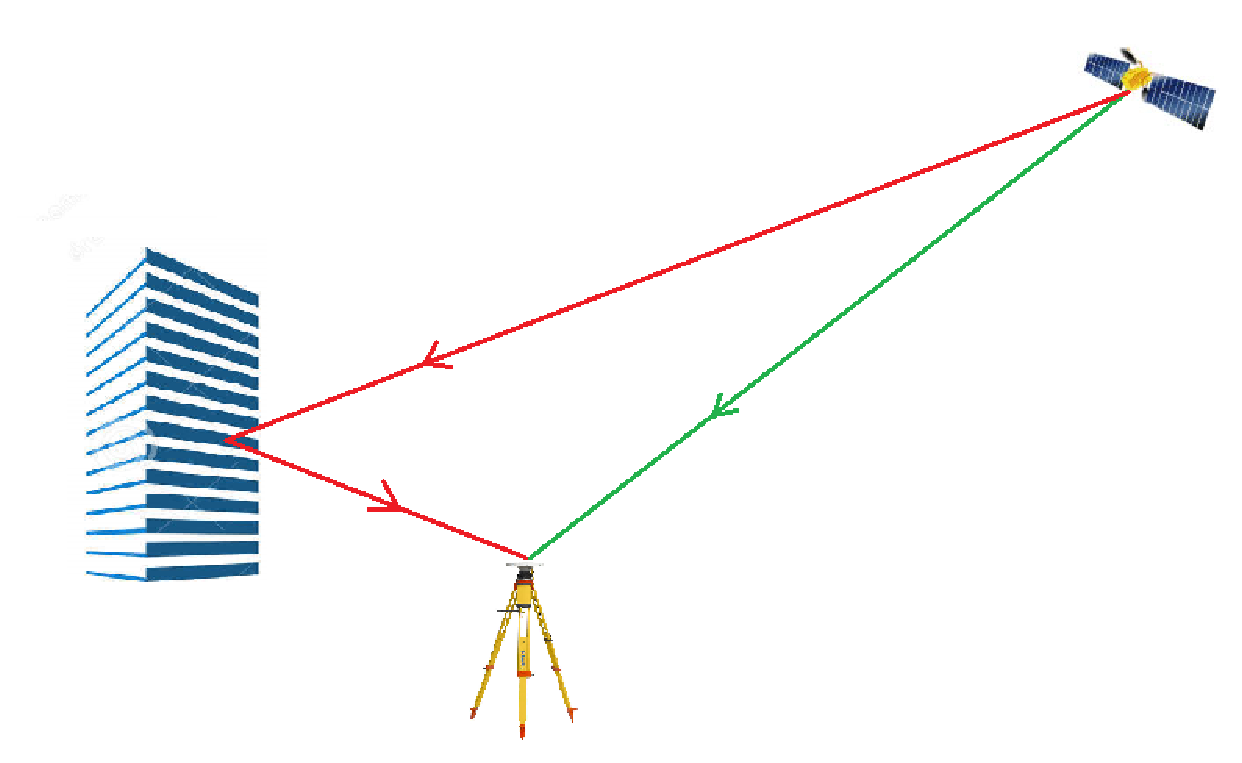
\includegraphics[scale=0.4]{fig/multipath_error.eps} 
	\caption{Multipath error}
	\label{FIG:multipath} 
\end{figure}


\subsubsection{Satellites geometry}

The satellites geometry is one of the main factors that affect the position accuracy. When the satellites are spread, the area of overlap of the signals is small, thus the uncertainty area is relatively small; vice versa, when the satellites are allocated close to each other, the area of overlap of the signals is larger (see figure \ref{FIG:sat_geometry}). The effect of satellites geometry is usually expressed by the DOP\footnote{Dilution Of Precision} index. The different parameters to quantify the goodness of the geometrical configurations are called PDOP\footnote{Position DOP}, HDOP\footnote{Horizontal DOP}, VDOP\footnote{Vertical DOP}, TDOP\footnote{Time DOP} and GDOP\footnote{Geometric DOP}. In particular GDOP index measures the overall accuracy:
%spostare dopo sta parte??

\begin{equation}
	GDOP = \sqrt{{\sigma_{x}}^{2}+{\sigma_{y}}^{2}+{\sigma_{z}}^{2}+{\sigma_{t}}^{2}}
	\label{eq:GDOP}
\end{equation}

where $\sigma$ is the root mean square of the 3D coordinates and time.

\begin{figure}[ht] 
	\centering
	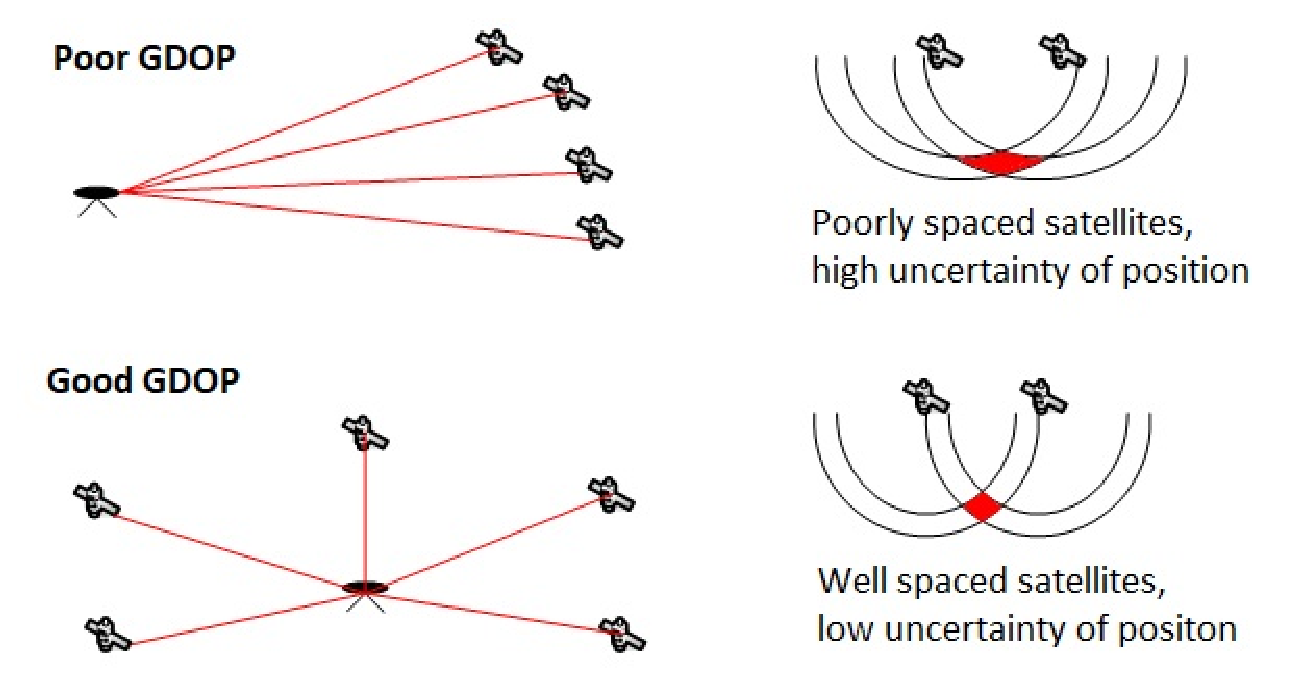
\includegraphics[scale=0.7]{fig/satellites_geometry.eps} 
	\caption{Overlapping signals' areas for spread and close satellites}
	\label{FIG:sat_geometry} 
\end{figure}


\subsection{Relative positioning}

Due to the previously introduced biases, the autonomous point positioning, i.e. \textit{absolute positioning}, can provide accuracy in the order of several meters. To achieve a better positioning precision and to overcome the presence of these errors, several positioning techniques have been developed, typically named \textit{relative positioning}.
Taking into account the main over-mentioned biases, the equation \ref{eq:phase_measure1} can be written as

\begin{equation}
	{\phi_{R}}^{S} = \frac{1}{\lambda}\cdot {\rho_{R}}^{S}(t) + f\cdot \left(\delta^{S}(t) - \delta_{R}(t)\right)+ {N_{R}}^{S}(t) + {I_{R}}^{S}(t) +{T_{R}}^{S}(t) + {E_{R}}^{S}(t)
	\label{eq:sat-receiver_errors}
\end{equation}

where ${I_{R}}^{S}$ is the ionospheric bias, ${T_{R}}^{S} $ is the tropospheric bias and $ {E_{R}}^{S} $ is the ephemerides bias.

Considering two generic receivers A and B, simultaneously observing the same satellite \textit{j}, as shown in figure \ref{FIG:relative_positioning}a, the observation equation \ref{eq:sat-receiver_errors}, could be written as:

%\begin{equation} 
%\begin{matrix} 
%{\phi_{A}}^{j}-f^{j}\cdot\delta^{j}(t) = \frac{1}{\lambda}\cdot {\rho_{A}}^{j}(t) + {N_{A}}^{j}(t) - f\cdot \delta_{A}(t) + {I_{A}}^{j}(t) +{T_{A}}^{j}(t) + {E_{A}}^{i}(t)\\ {\phi_{B}}^{j}-f^{j}\cdot\delta^{j}(t) = \frac{1}{\lambda}\cdot {\rho_{B}}^{j}(t) + {N_{B}}^{j}(t) - f\cdot \delta_{B}(t) + {I_{B}}^{j}(t) +{T_{B}}^{j}(t) + {E_{B}}^{i}(t) \end{matrix} 
%\\
%\label{eq:SingleDifferences1}
%\end{equation}

\begin{equation}\begin{split} 
		{\phi_{A}}^{j}-f^{j}\cdot\delta^{j}(t) & = \frac{1}{\lambda}\cdot {\rho_{A}}^{j}(t) + {N_{A}}^{j}(t) - f\cdot \delta_{A}(t) + {I_{A}}^{j}(t) +{T_{A}}^{j}(t) + {E_{A}}^{i}(t)\\ {\phi_{B}}^{j}-f^{j}\cdot\delta^{j}(t) & = \frac{1}{\lambda}\cdot {\rho_{B}}^{j}(t) + {N_{B}}^{j}(t) - f\cdot \delta_{B}(t) + {I_{B}}^{j}(t) +{T_{B}}^{j}(t) + {E_{B}}^{i}(t) 
		\label{eq:SingleDifferences1}
	\end{split}
\end{equation}

The difference between the two equations in \ref{eq:SingleDifferences1} is

\begin{equation}\begin{split}
		{\phi_{B}}^{j}-{\phi_{A}}^{j} = \frac{1}{\lambda}\cdot \left({\rho_{B}}^{j}(t)-{\rho_{A}}^{j}(t)\right)+ & {N_{B}}^{j}(t)-{N_{A}}^{j}(t)- f^{j}\cdot \left(\delta_{B}(t)-\delta_{A}(t)\right) + \\ {I_{B}}^{j}(t)- {I_{A}}^{j}(t) +{T_{B}}^{j}(t) & - {T_{A}}^{j}(t) + {E_{B}}^{j}(t)-{E_{A}}^{j}(t)
		\label{eq:eq:SingleDifferences1}
	\end{split}
\end{equation}
% la & nelle due righe della equazione serve per dirgli come incolonnarle (le due & corrisponderanno)

This process is called \textit{single differences} (SD). It is important to note that the single differences lead to the elimination of the terms $f^{j}\cdot\delta{j}(t)$ , which are related to the non-synchronization of the satellite’s clock and are common to the two equations in the hypothesis that the two receivers are observing the same satellite $j$.
While the term depending on the satellite clock bias is eliminated by means of single differences, equation \ref{eq:SingleDifferences1} is still sensitive to both receivers clock errors ($\delta_{A}$ and $\delta_{B}$ are still present in the equation).
Introducing the following notations:

\begin{equation} 
	\begin{matrix} 
		{\phi_{AB}}^{j}={\phi_{B}}^{j}-{\phi_{A}}^{j}\\ {\rho_{AB}}^{j}={\rho_{B}}^{j}-{\rho_{A}}^{j}\\{N_{AB}}^{j}={N_{B}}^{j}-{N_{A}}^{j}\\{\delta_{AB}}^{j}={\delta_{B}}^{j}-{\delta_{A}}^{j}\end{matrix}
	\\
	\label{eq:notation1}
\end{equation}

Equation \ref{eq:SingleDifferences1} turns into:

\begin{equation}
	{\phi_{AB}}^{j}(t)=\frac{1}{\lambda}\cdot {\rho_{AB}}^{j}(t)+{N_{AB}}^{j}(t)-f^{j}\cdot{\delta_{AB}}^{j}(t)+\Delta {I_{AB}}^{j}(t)+\Delta {T_{AB}}^{j}(t)+\Delta {E_{AB}}^{j}(t)
	\label{eq:double_diff0}
\end{equation}

Considering two generic receivers A and B, simultaneously observing the same two satellites $i $ and $j$, as reported in figure \ref{FIG:relative_positioning}b, it is possible to write two single differences equations, one for each satellite:

\begin{equation} 
	\begin{split} 
		{\phi_{AB}}^{i}(t)&=\frac{1}{\lambda}\cdot {\rho_{AB}}^{i}(t)+{N_{AB}}^{i}(t)-f^{i}\cdot{\delta_{AB}}^{i}(t)+\Delta {I_{AB}}^{i}(t)+\Delta {T_{AB}}^{i}(t)+\Delta {E_{AB}}^{i}(t)\\ {\phi_{AB}}^{j}(t)&=\frac{1}{\lambda}\cdot {\rho_{AB}}^{j}(t)+{N_{AB}}^{j}(t)-f^{j}\cdot{\delta_{AB}}^{j}(t)+\Delta {I_{AB}}^{j}(t)+\Delta {T_{AB}}^{j}(t)+\Delta {E_{AB}}^{j}(t)  
		\label{eq:double_diff1}
	\end{split}
\end{equation}

Assuming that the two signal frequencies are equal, the difference between the two equations in \ref{eq:double_diff1} is

\begin{equation} 
	\begin{split}
		{\phi_{AB}}^{j}(t)-{\phi_{AB}}^{i}(t) & = \frac{1}{\lambda}\cdot \left({\rho_{AB}}^{j}(t)-{\rho_{AB}}^{i}(t)\right)+{N_{AB}}^{j}(t)- {N_{AB}}^{i}(t) \\ + \nabla\Delta & {I_{AB}}^{ij}(t)  + \nabla \Delta {T_{AB}}^{ij}(t)+\nabla \Delta {E_{AB}}^{ij}(t)
		\label{eq:double_diff2}
	\end{split}
\end{equation}

The symbols $\nabla \Delta$ indicate the double differences operated on the ionospheric, tropospheric and ephemerides biases. This process is called \textit{double differences} (DD). It is important to note that the double differences lead to the elimination of the terms $f^{j}\cdot {\delta_{AB}}^{j}(t)$, which are related to the receivers’ clock bias and are common to the two equations in the hypothesis that the two signal frequencies are the same.

Introducing the notations:
\begin{equation} 
	\begin{matrix} 
		{\phi_{AB}}^{ij}={\phi_{AB}}^{j}-{\phi_{AB}}^{i}\\ {\rho_{AB}}^{ij}={\rho_{AB}}^{j}-{\rho_{AB}}^{i}\\{N_{AB}}^{ij}={N_{AB}}^{j}-{N_{AB}}^{i}\end{matrix}
	\\
	\label{eq:notation2}
\end{equation}

Equation \ref{eq:double_diff2} turns into

\begin{equation}
	{\phi_{AB}}^{ij}(t)=\frac{1}{\lambda}\cdot {\rho_{AB}}^{ij}(t)+{N_{AB}}^{ij}(t)+ \nabla\Delta{I_{AB}}^{ij}(t)  + \nabla \Delta {T_{AB}}^{ij}(t)+\nabla \Delta {E_{AB}}^{ij}(t)
	\label{eq:triple_diff0}
\end{equation}

To remove the time independent ambiguities, two double differences referring to two different epochs could be used, obtaining the \textit{triple differences} (see figure \ref{FIG:relative_positioning}c). Considering two epochs $t_{1}$ and $t_{2}$, it is possible to write two double differences equations, one for each epoch

\begin{equation} 
	\begin{split} 
		{\phi_{AB}}^{ij}(t_{1})&=\frac{1}{\lambda}\cdot {\rho_{AB}}^{ij}(t_{1})+{N_{AB}}^{ij}(t_{1})+\nabla\Delta {I_{AB}}^{ij}(t_{1})+\nabla\Delta{T_{AB}}^{ij}(t_{1})+\nabla\Delta{E_{AB}}^{ij}(t_{1})\\ {\phi_{AB}}^{ij}(t_{2})&=\frac{1}{\lambda}\cdot {\rho_{AB}}^{ij}(t_{2})+{N_{AB}}^{ij}(t_{2})+\nabla\Delta {I_{AB}}^{ij}(t_{2})+\nabla\Delta{T_{AB}}^{ij}(t_{2})+\nabla\Delta{E_{AB}}^{ij}(t_{2})
		\label{eq:triple_diff1}
	\end{split}
\end{equation}

For baselines not exceeding 10-15 km, it is always possible to consider the space correlated ionospheric, tropospheric and ephemerides residuals equal to zero, assuming that the biases are equivalent. The difference between the two equations in \ref{eq:triple_diff2} is

\begin{equation} 
	{\phi_{AB}}^{ij}(t_{2})-{\phi_{AB}}^{ij}(t_{1})=\frac{1}{\lambda}\cdot \left({\rho_{AB}}^{ij}(t_{2})-{\rho_{AB}}^{ij}(t_{1})\right)
	\label{eq:triple_diff2}
\end{equation}

It is important to note that the triple differences lead to the elimination of the terms ${N_{AB}}^{ij}$, which is related to the unknown phase ambiguities. The triple differences is often considered a pre-processing technique to obtain good quality approximate positions for the double differences solution, thanks to the linear combination, which let to remove the ambiguity.

\begin{figure}[ht] 
	\centering
	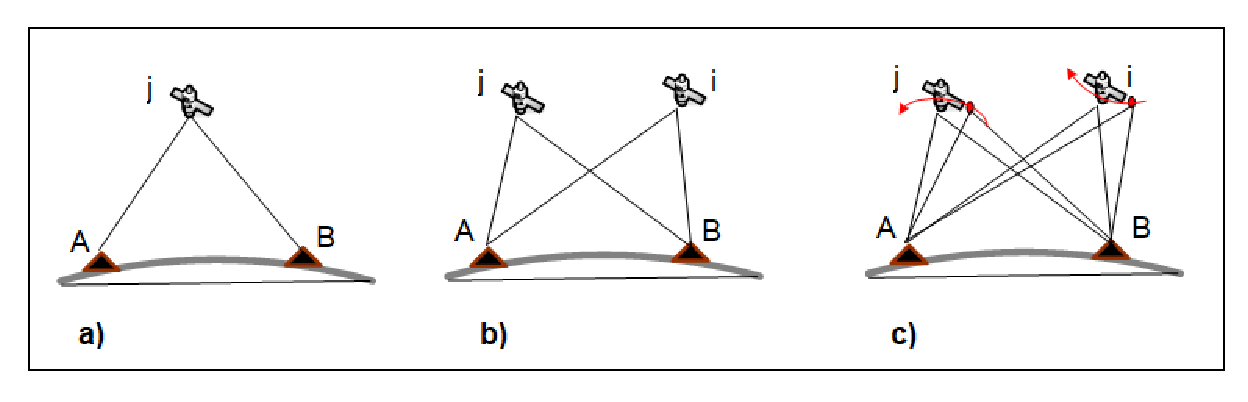
\includegraphics[scale=0.8]{fig/relative_positioning.eps} 
	\caption{Relative positioning assets}
	\label{FIG:relative_positioning} 
\end{figure}

\subsection{RTK positioning}

In general, the determination of the absolute position is less accurate than the relative positioning
between two stations. This is due to the high correlation among the acting errors. To minimize the impact of errors decorrelated with distance, the coordinates
are estimated with respect to a known reference station.
With origin dating back to the mid-1990s, Real Time Kinematics (RTK) is a differential GNSS technique which provides high positioning performance in the vicinity of a base station. The technique is based on the use of carrier measurements and the transmission of corrections from the base station, whose location is well known, to the rover, so that the main errors that drive the stand-alone positioning cancel out. A RTK base station covers a service area spreading about 10 or 20 kilometres, and a real time communication channel is needed connecting base and rover. RTK, which achieves performances in the range of a few centimetres, is a technique commonly used in surveying applications.

From an architectural point of view, RTK consists of a base station, one or several rover users, and a communication channel with which the base broadcasts information to the users in real time.
The technique is based on the following high-level principles:

\begin{itemize}
    \item In the neighbourhood of a clean-sky location, the main errors in the GNSS signal processing are constant, and hence they cancel out when differential processing is used. This includes the error in the satellite clock bias, the satellite orbital error, the ionospheric delay and the tropospheric delay. The main errors left without correction are multipath, interference and receiver thermal noise. Of the errors listed above, the only one which is truly constant with respect to the user location is the satellite clock bias; the rest will show a given dependency with the location as the rover moves away from the base station, being the tropospheric error the first to be fully de-correlated in a few kilometres from the base.
    \item The noise of carrier measurements is much smaller than the one of the pseudo-code measurements. The typical error of code pseudorange measurements is around 1 m, to compare with 5 mm for carrier phase measurements. However, the processing of carrier measurements is subject to the so-called carrier phase ambiguity, an unknown integer number of times the carrier wave length, that needs to be fixed in order to rebuild full range measurements from carrier ones.
    \item The phase ambiguities can be fixed using differential measurements between two reference stations. There are different techniques available to fix them, some based on single frequency measurements with long convergence times, other taking benefit of dual frequency observables with shorter convergence. In general, the techniques either depend on a high precision knowledge of the ionosphere, or assume that the two stations are close enough so that the ionospheric differential delay is negligible when compared with the wave-length of the carriers, around 20 cm. The latter is the approached followed in RTK, limiting the service area to 10 or 20 km; the former is used in WARTK (Wide Area RTK) to cover big service areas with base stations separated around hundreds of kilometres away. The RTK approach needs continuity in the tracked measurements to avoid re-initialization of the phase-ambiguity filters; this is a severe limitation in urban environments due to the big number of obstructions.
\end{itemize}

The base station broadcasts its well-known location together with the code and carrier measurements at frequencies L1 and L2 for all in-view satellites. With this information, the rover equipment is able to fix the phase ambiguities and determine its location relative to the base with high precision. By adding up the location of the base, the rover is positioned in a global coordinate framework.
The RTK technique can be used for distances of up to 10 or 20 kilometres, yielding accuracies of a few centimetres in the rover position, to be compared with 1 m that is achieved with code-based differential GPS. Because of its high precision in controlled environments, RTK is extensively used in surveying applications.
As stated in the previous section, one of the main problems in the RTK technique is fixing the phase ambiguities. The RTK Algorithm is based on double differenced observables that can eliminate selective availability effects as well as other biases (equation \ref{eq:double_diff2}). In this model receiver and satellite clock offsets and hardware biases cancel out. The single difference ambiguities difference $N_{AB}^{j}(t)-N_{AB}^{i}(t)$ is commonly parameterized as a new ambiguity parameter $N_{AB}^{ij}(t)$. The advantage of double differencing is that the new ambiguity parameter $N_{AB}^{ij}(t)$ is an integer because the non-integer terms in the GPS carrier phase observation, due to clock and hardware delays in the transmitter and receiver, are eliminated.
Although it would be possible to estimate the double difference ambiguity using a float approach instead of an integer one, this would lead to dm-level accuracy instead of cm-level. Hence, standard RTK fixes the ambiguities to integer.

Concerning the ambiguity fixing procedure, normally this is done in three steps \cite{Eissfeller:2002}:
\begin{itemize}
\item The ambiguities are first fixed to float numbers using standard least-square techniques.
\item The set of integer ambiguities is set to the one that optimizes the residuals in the surroundings of the float solution.
\item The carrier measurements are corrected with the integer ambiguities, and they are used to obtain the relative position of the rover to the base station.
\end{itemize}

Of these three steps, the second one is quite complex, because the float ambiguity covariance ellipsoid in the measurement space is extremely elongated. As a consequence, the brute-force search process is inefficient, normally beyond the computational capabilities of the rover equipment. Several techniques have been developed to deal with this problem \cite{Laurichesse:2006, Ge:2008, Collins:2008, Teunissen_ar1995, chang2005}.







\subsection{Network-RTK positioning}

One of the major issues related to RTK applications is that the influence of some errors, like
orbit, ionosphere and troposphere, grows with the distance from the reference station. Furthermore,
the impact of the atmospheric error sources depends on solar activity and weather
conditions, which makes the definition of a maximum favorable distance complicated. In order
to overcome this distance-dependent effect, the Network RTK (NRTK) technique has been
developed. The CORS (Continuosly Operating Systems) availability allows the estimate of the state space for the area covered by
the network of reference stations. As a consequence, corrections for a user within the area covered
by the network can be generated and transmitted. Commonly used procedures for NRTK
are the concept of area correction parameters (FKP from the German word Flaechen Korrektur
Parameter), Master Auxiliary Concept (MAC), and Virtual Reference Station (VRS). 
The FKP approach represents additional corrections for the distance-dependent errors by
utilizing a polynomial parametrization to describe the influence of any rover position in a certain
area. These corrections are transmitted in addition to the range corrections of the reference
station considered.
The MAC approach consists in the transmission of observation data of a master station
and correction differences between master and auxiliary stations. The rover can re-construct
the observation data of the auxiliary stations (except a common clock term) and decide how
to use master and auxiliary data for its location.
The VRS approach needs a two-way communication link between rover and network. The
rover communicates their approximate location to the network, which interpolates the observations of all the network station to create and send to the rover a Virtual Reference Station in its proximity. 
